\clearpage
\section{Overview of the sensing and power-management custom board} \label{sec:custom}

This section helps you to better understand the different blocks present on the \texttt{sensing and power management} board and how you can use it throughout this project. Figure \ref{fig:pcb-overview} gives a simplified overview of the custom board while the full schematic is given in Fig \ref{fig:schematic}. Please do not try to figure out how it works without having read carefully this guide beforehand. \\

You will not need to master all parts of this board for the first weeks, but it is important that you get aware of the functionalities available on the board and what to be careful with. A good practice to keep in mind is to \textit{never} power a system (i.e. a board, a test setup or whatever) if you have not checked in advance that everything seemed to be properly connected and set. Having a quick visual check and being focused on what you are doing is critical not to damage the hardware.

\begin{figure}[h!]
    \centering
    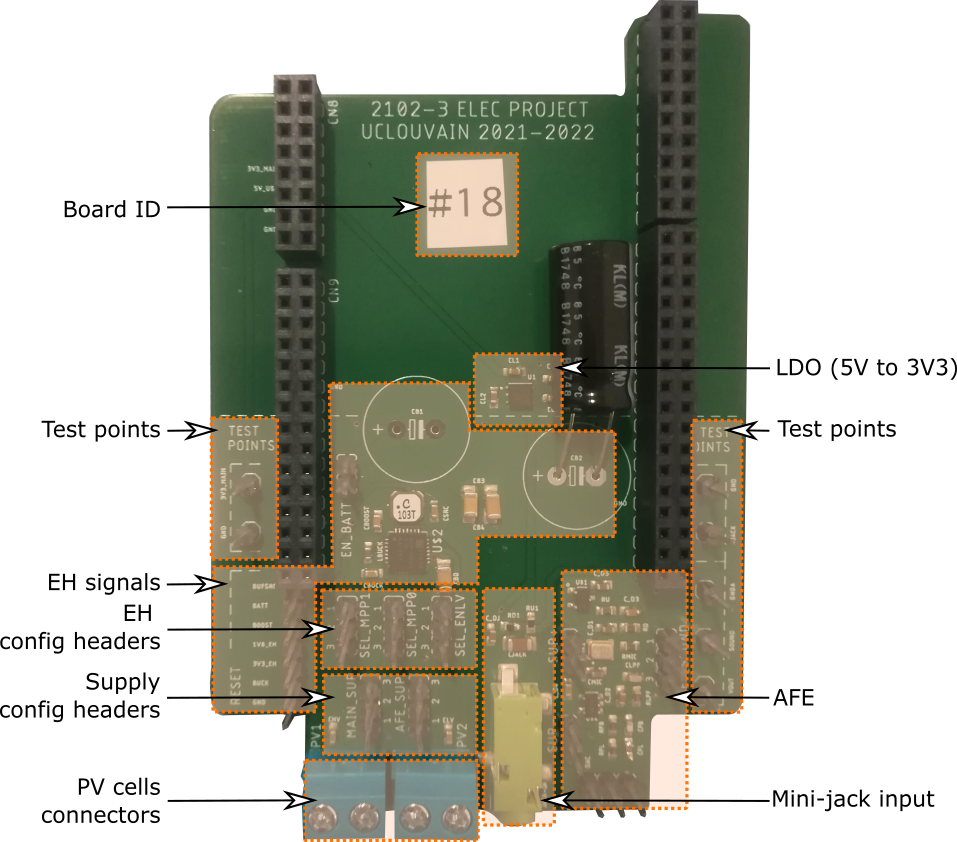
\includegraphics[width=0.8\textwidth]{figs/pcb-overview.png}
    \caption{Simplified overview of the \texttt{sensing and power-management} board, block by block.}
    \label{fig:pcb-overview}
\end{figure}

\clearpage
\subsection{Test points}

These headers allow you to monitor several useful signals on the board. Typically, you have easy access to the following signals:

\begin{table}[h!]
    \centering
    \begin{tabular}{l l }
         \textbf{Header} & \textbf{Description} \\
         \toprule
         3V3\_MAIN & Main power supply of the boards \\
                   & It supplies also the MCU on the \texttt{STM32 NUCLEO} MCU board  \\
         GND & Ground \\
         JACK & Signal at the output of the HPF, after the mini-jack \\
         SOUND & Signal sent to the ADC on the \texttt{STM32 NUCLEO} MCU board \\
         VOUT & Signal at the output of the amplifier (before the LPF) \\
    \end{tabular}
    \caption{Test points signals}
    \label{tab:TP-signals}
\end{table}

\subsection{EH signals}

These headers allow you to monitor EH signals on the board. Typically, you have easy access to the following signals:

\begin{table}[h!]
    \centering
    \begin{tabular}{l l }
         \textbf{Header} & \textbf{Description} \\
         \toprule
         BUFSRC & Voltage on the BUFSRC node \\
         BATT & Voltage on the storage capacitor(s) \\
         BOOST & Voltage on the BOOST node \\
         1V8\_EH & LVOUT output \\
         3V3\_EH & HVOUT output \\
         BUCK & Voltage on the BUCK node \\
         GND & Ground
    \end{tabular}
    \caption{Test points signals}
    \label{tab:TP-signals}
\end{table}

By default, a $150 \mu F$ capacitor is used as storing device for the EH part. To this minimum, additional storage devices can be added as shown in the schematic of the board in Fig. \ref{fig:schematic} (not all of them have be soldered on the board yet). To connect these supplementary capacitors, connect the EN\_BATT jumper.

\subsection{EH config headers}

These headers allow you to configure the EH part of the board as described in Table \ref{tab:EH-headers}. Please refer to the AEM10941 datasheet for more details about the maximum power point (MPP) tracking configuration and the outputs available (\url{https://www.mouser.be/datasheet/2/1087/e_peas_AEM10941_datasheet_energy_harvesting-2325372.pdf}).

\begin{table}[h!]
    \centering
    \begin{tabular}{l c l}
         \textbf{Header} & \textbf{Config: Jumper on Pin 2 + Pin\dots} & \textbf{Description} \\
         \toprule
         SEL\_MPP0 (2) & 1 & Tied down, i.e. GND = 0 V  \\
                       & 3 & Tied up, i.e. BUCK = 3.3 V \\
         SEL\_MPP1 (2) & 1 & Tied down, i.e. GND = 0 V  \\
                       & 3 & Tied up, i.e. BUCK = 3.3 V \\
         SEL\_ENLV (2) & 1 & LVOUT disabled \\
                       & 3 & LVOUT enabled (1.8 V)\\
    \end{tabular}
    \caption{Available configurations for the EH headers}
    \label{tab:EH-headers}
\end{table}

\subsection{Supply config headers}

These headers allow you to configure the supplies (of the boards and AFE parts) as described in Table \ref{tab:supply-headers}.

\begin{table}[h!]
    \centering
    \begin{tabular}{l >{\centering}p{8em} l}
         \textbf{Header} & \textbf{Config: Jumper on Pin 2 + Pin\dots} & \textbf{Description} \\
         \toprule
         MAIN\_SUP (2) & 1 & Select the 3V3\_EH source as the main power supply \\
                   & 3 & Select the 3V3\_USB source as the main power supply \\
         AFE\_SUP (2) & 1 & Select the 1V8\_EH as power supply for the AFE  \\
                   & 3 & Select the 3V3\_MAIN source as power supply for the AFE \\
    \end{tabular}
    \caption{Available configurations for the supply headers}
    \label{tab:supply-headers}
\end{table}

\subsection{AFE}

The schematic of the AFE can be found in Fig. \ref{fig:schematic}. The annotations provided on this figure should help you to better understand the function of each part of the circuit. Feel free to zoom-in to see details properly ! Useful datasheets for specific components are also provided on the Moodle in the folder \texttt{Technical resources}. \\

The frequency response of the AFE simulated in LTSpice is provided in Fig. \ref{fig:bode_AFE}. $V_{VOUT}$ and $V_{LP}$ are respectively the output of the amplifier and the output of the additional low pass filter, as shown in Fig. \ref{fig:schematic}. \\

In order to enable the AFE part on the custom board, you must connect the jumpers SUP+ and SUP-. The SEL\_SOUND header can be used to configure which signal you send to the ADC of the MCU, as described in Table \ref{tab:afe-headers}.

\begin{table}[h!]
    \centering
    \begin{tabular}{l >{\centering}p{8em} p{0.5\textwidth}}
         \textbf{Header} & \textbf{Config: Jumper on Pin 2 + Pin\dots} & \textbf{Description} \\
         \toprule
         SEL\_SOUND (2) & 1 & Select the JACK signal as the input for the ADC \\
                   & 3 & Select the output of the LPF signal of the AFE as the input for the ADC
    \end{tabular}
    \caption{Available configurations for the supply headers}
    \label{tab:afe-headers}
\end{table}

The CTRLS headers are currently not used in the design of the AFE. Consequently, they have no impact on the AFE behavior. However, keep in mind that in these three headers, one is a DAC and the two other ones are GPIO connections to the MCU. That might be useful in the second part of the project (LELEC2103) if you want to design a custom AFE.



% \begin{figure}[h!]
%     \centering
%     \includegraphics[width=1\textwidth]{figs/afe.png}
%     \caption{Analog Front-End (AFE) schematic.}
%     \label{fig:afe}
% \end{figure}

\clearpage
\begin{figure}[h!]
    \centering
    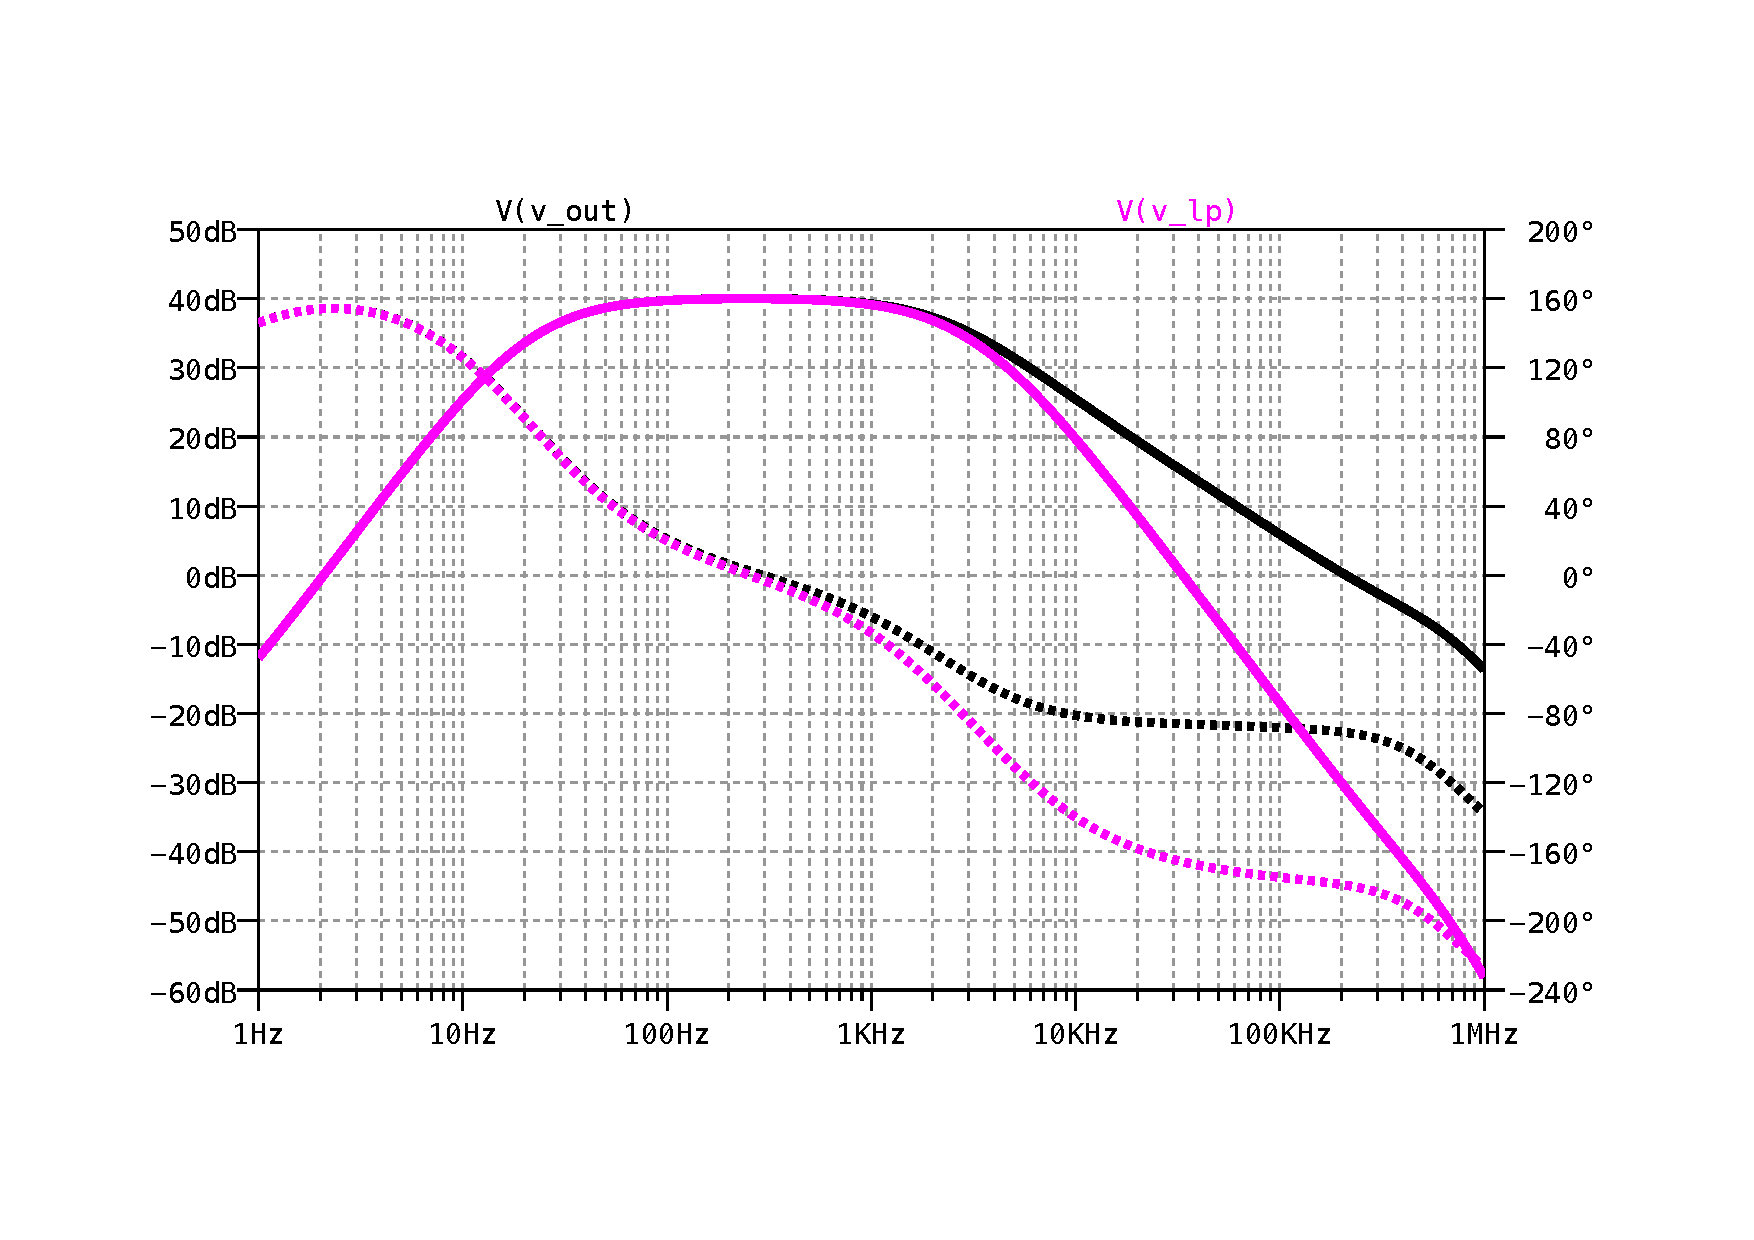
\includegraphics[scale=0.8, angle=90]{figs/bode_AFE.pdf}
    \caption{LTSpice results for the simulation of the AFE. Note: the microphone is not modeled in this simulation. The LTSpice model provided by Microchip has been used for the MCP6231.}
    \label{fig:bode_AFE}
\end{figure}

\clearpage
\subsection{Schematic of the sensing and power-management board}

\begin{figure}[h!]
    \centering
    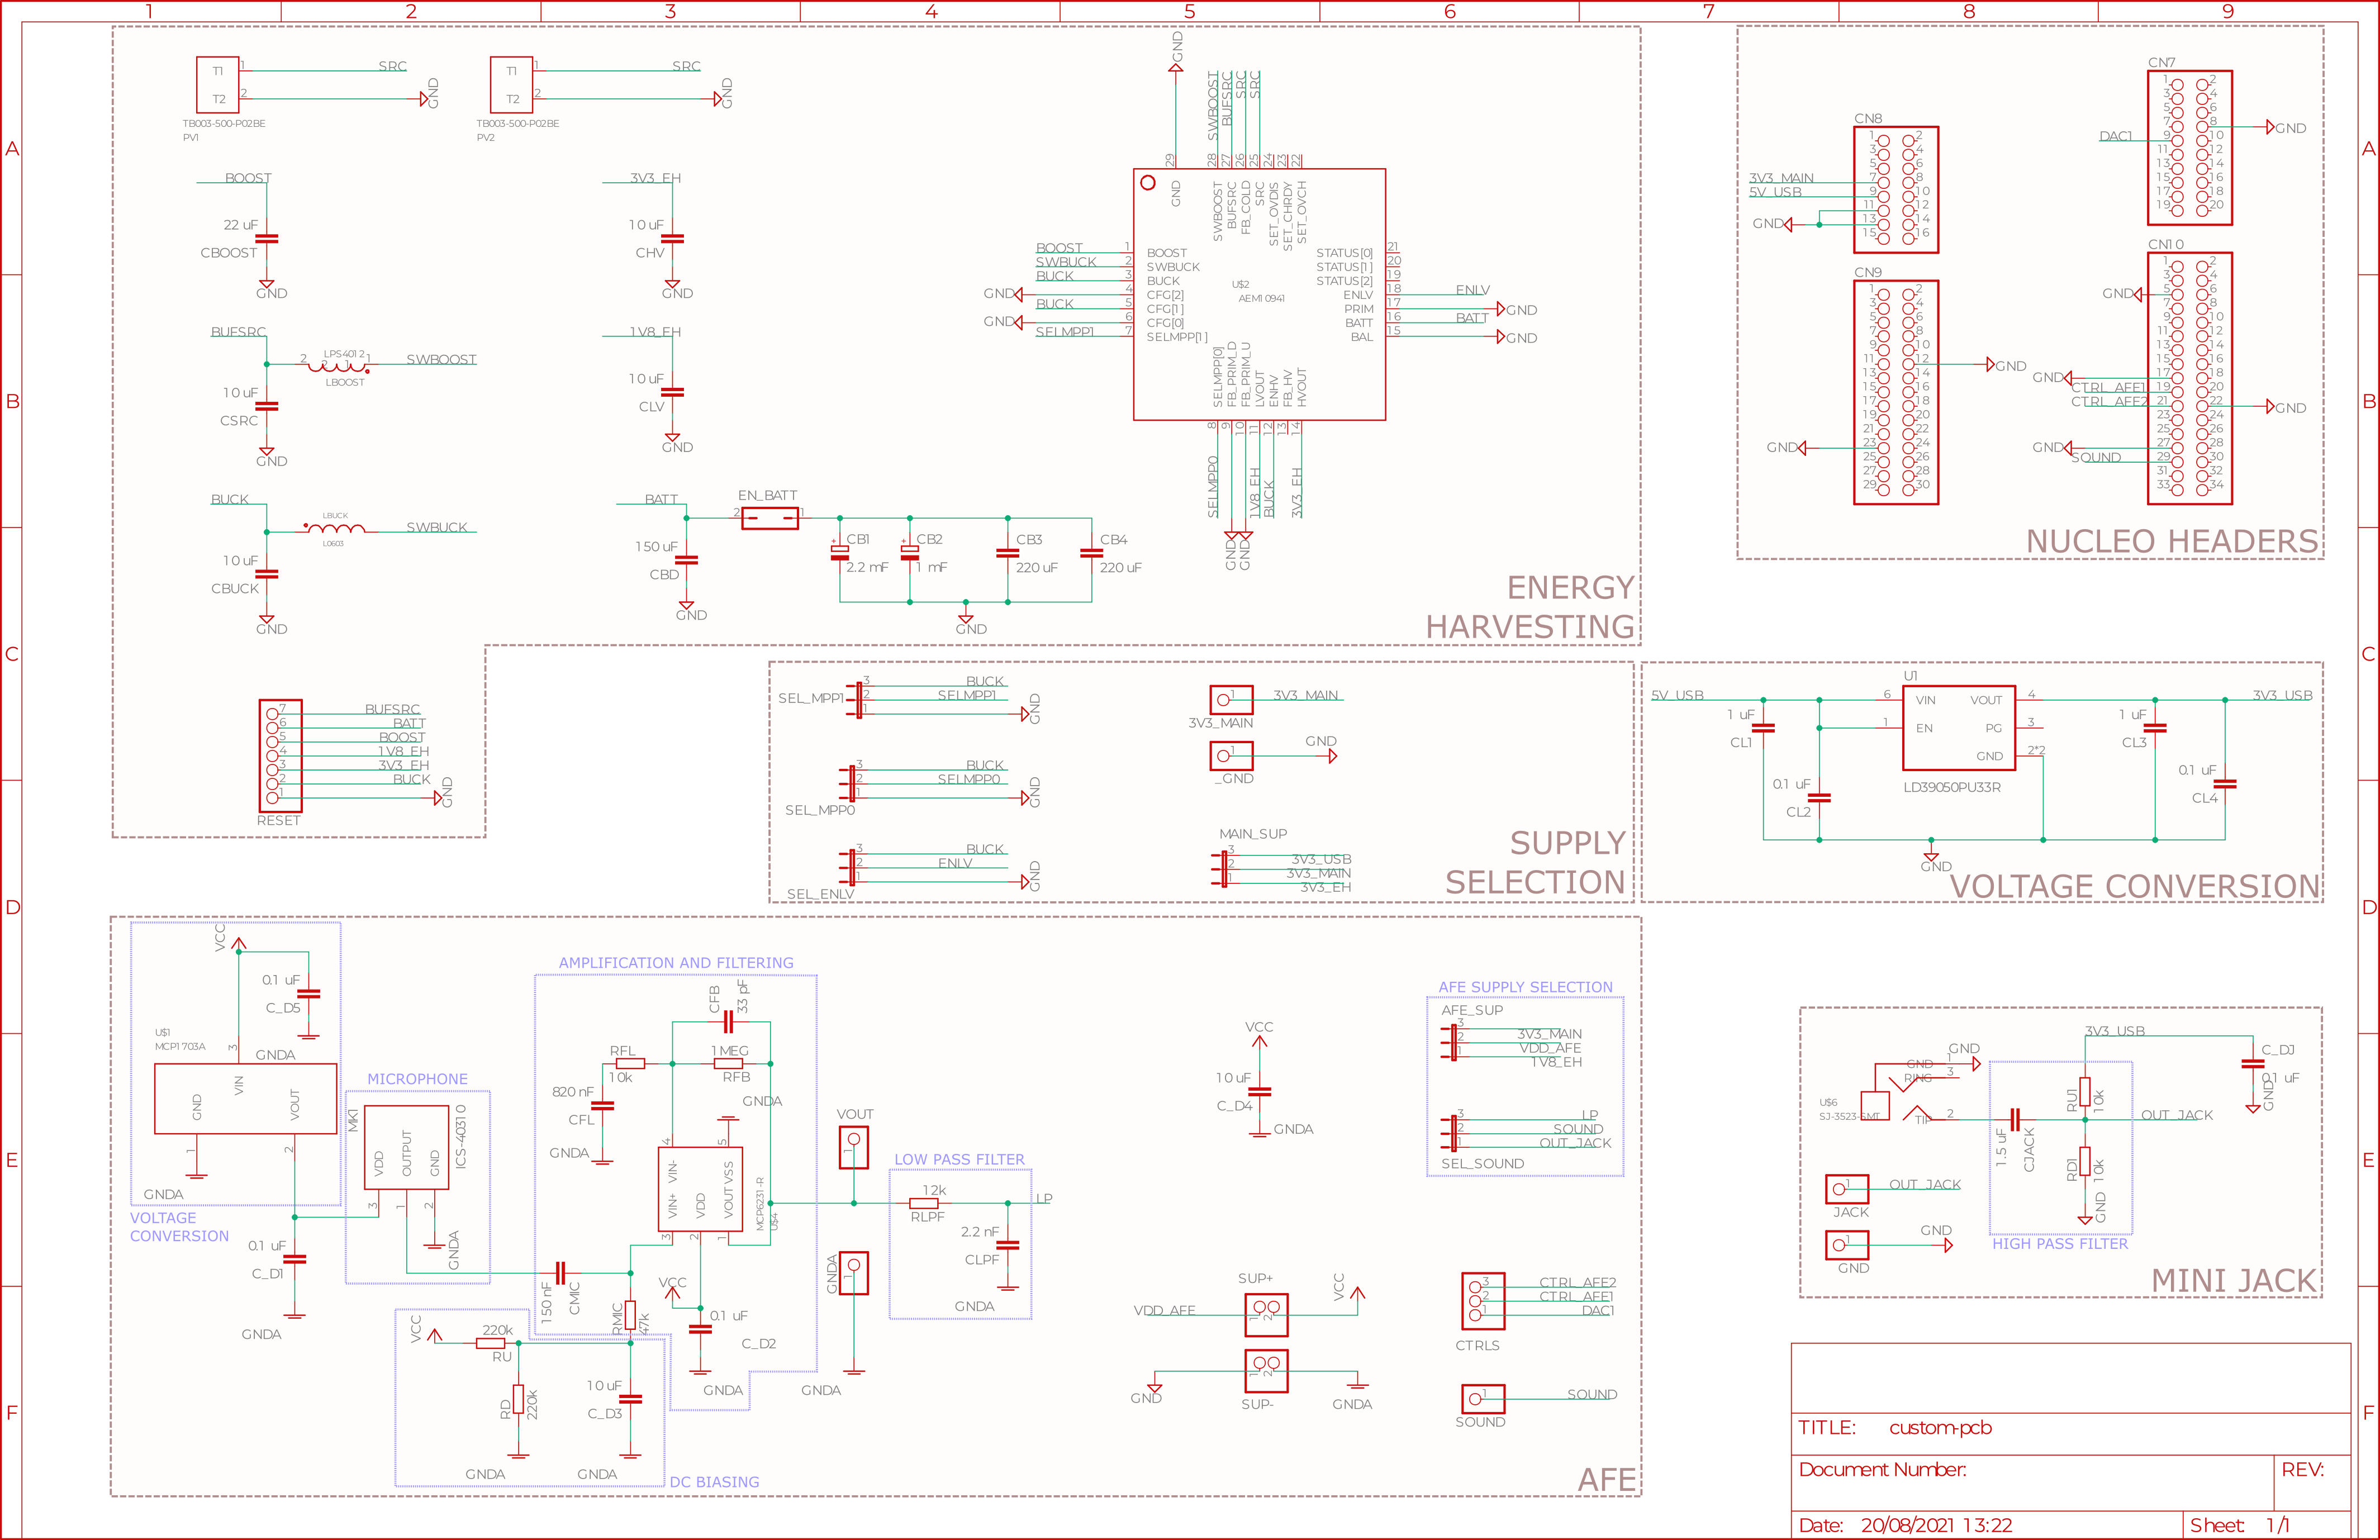
\includegraphics[scale=1, angle=90]{figs/schematic.png}
    \caption{Schematic of the \texttt{sensing and power-management} board.}
    \label{fig:schematic}
\end{figure}
